\section{Methods}
\subsection{Subjects}
42 healthy subjects, 21 female and 21 male were recruited (age: 23.93 $\pm$ 2.74 years, BMI: 23.66 $\pm$ 3.28). Subjects with ongoing meditation practice, acute or chronic pain, neurological, musculoskeletal or mental illness, pregnancy or taking medications that might influence their response to pain were excluded.

\subsection{Study design}
A controlled trial was designed, whereby the subjects were assigned into a control and treatment group with an equal gender distribution, as illustrated in \autoref{fig:studydesign}.

\begin{figure}[H]
\centering
%\caption{} \vspace{-.25cm}
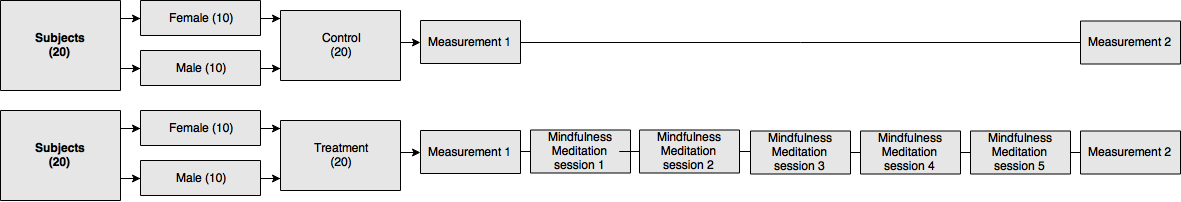
\includegraphics[width=1\columnwidth]{../figures/studydesign.png}
\caption{Parallel study design, whereby subjects were assigned to either treatment or control group, striving an equal gender distribution. The treatment group was meditating on 5 consecutive days between the measurements, whilst the control group continued their normal routine.}
\label{fig:studydesign}
\end{figure} 

\noindent 
The subjects of the treatment group practiced 20 minutes mindfulness FA meditation on 5 consecutive days between the two measurements, while the subjects of the control group continued their normal routine. The same time interval between the measurement sessions was used for the two groups.

\subsection{Measurements}%Experimental Procedure
The testing point, as shown in \autoref{fig:trapezius}, was marked at the right upper trapezius between the acromion and 7th cervical vertebra to ensure reliable and rapid location during the experimental procedure. 

Pressure pain threshold and pressure pain tolerance were measured with an algometer (Wagner Force Ten™ Digital force Gage). Three repetitions with a 5 minutes resting period in between were conducted. The examiner was blinded during the measurements to avoid bias. The mean of the three repetitions, was computed. 

\begin{figure}[H]
\centering
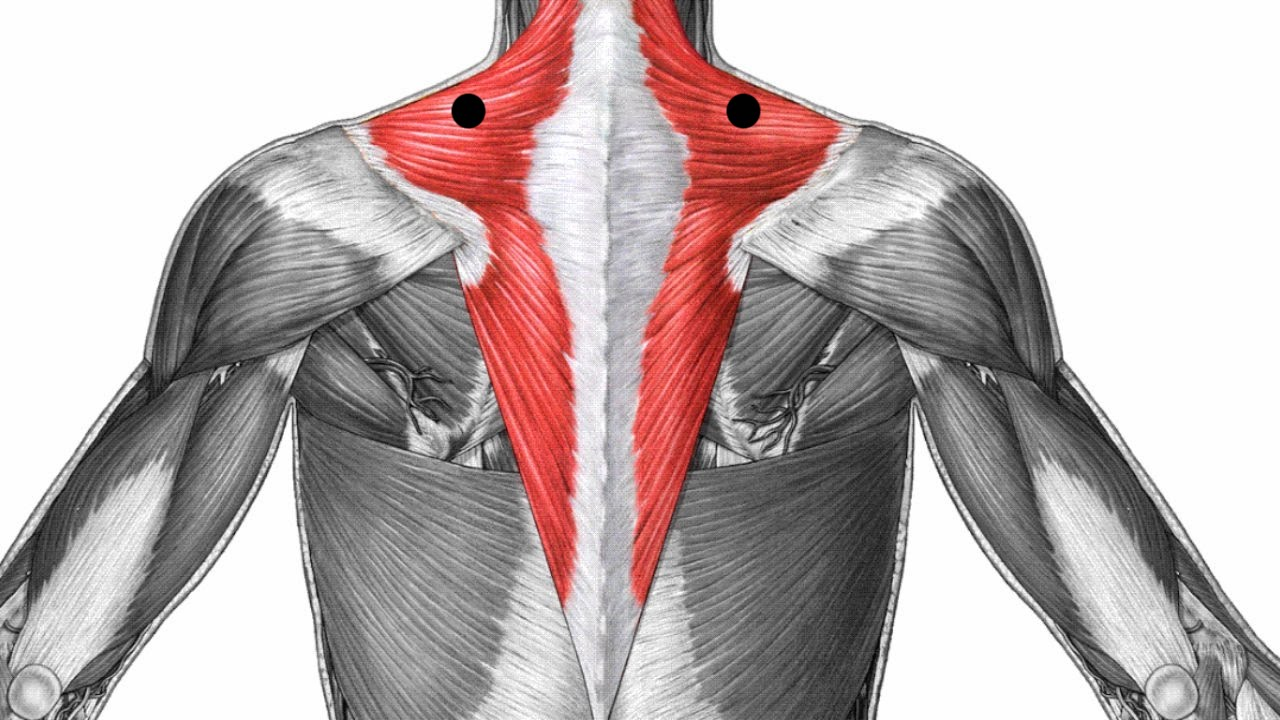
\includegraphics[width=.7\columnwidth]{../figures/trapezius}
\caption{Testing point on the right upper trapezius.}
\label{fig:trapezius}
\end{figure} \vspace{-.5cm}

%The treatment group practiced 20 minutes mindfulness meditation on 5 consecutive days. After the last meditation session the second measurement was conducted likewise the baseline measurement.
%The subjects of the control group continued their normal routine. The same time interval between baseline and second measurement was used for the subjects of the control group.

\subsection{Meditation Technique}
The treatment group practice short-term mindfulness FA meditation with 20 minutes of meditation on 5 consecutive days. To ensure same meditation conditions, a guided meditation in form of an audio file was used. The used meditation technique was FA focusing on the flow of breath. A short oral introduction to mindfulness FA meditation was provided before the first meditation session. 

\subsection{Data Analysis}
%At first the normality of the data sample was evaluated with a Shapiro-Wilk test. According to the outcome of the Shapiro-Wilk test, for comparison of treatment and control group with regards to threshold and tolerance of first and second measurement a two-way mixed ANOVA was applied. For comparison of the groups with regards to the difference in threshold and tolerance as a percentage of first and second measurement a t-test was applied.

At first the normality of the data samples was evaluated with a Shapiro-Wilk test and the equality of variances was evaluated with a Levene's test. 

According to the outcome of the Shapiro-Wilk test and the Levene’s test, ANOVA and t-test were chosen. The two-way mixed ANOVA was used, whereby factor 1 denotes the group of subjects, either treatment or control, and factor 2 denotes the measurement session, either the first (Pre) or the second (Post). Therewith the statistical significance of two variations was evaluated, the between-subjects variation in factor 1 and the within-subjects variation in factor 2. \cite{Mooi2018} Threshold and tolerance have been analyzed with separate two-way mixed ANOVAs.

The t-test was used to compare the changes in threshold and tolerance between the measurement sessions of treatment and control group. Therefore the relative difference (Improvement) in threshold and tolerance between Pre and Post was calculated for each subject. A t-test was applied to the Improvements to test the mean difference between treatment and control group’s Improvement. \cite{Mooi2018} Threshold and tolerance Improvements have been analyzed separately.


